% Implementation 
\chapter{Implementation}
\label{sec:implement}
This section briefly overviews the experimental setup and aims to motivate the choice of datasets, libraries, and frameworks.

\section{Scope and Limitations}
\label{sec:implement:scope}
Our research is concerned only with graph-level prediction tasks on two types of \ac{gnn}, \ac{gcn} and \ac{gin}.
We implemented both networks as described by \citet{Kipf2017} and \citet{Xu2019} respectively.
\Ac{gdc} is implemented like it is described in \ref{eq:relaxed} as it allows for better time and space complexity, which is the same reason this equation was originally used and evaluated by \citet{Hasanzadeh2020}. We perform our experiments using five datasets, all within the molecular realm. \cite{Hu2020} Two of the datasets are for classification and the rest for regression tasks. Apart from evaluating \ac{gdc}, we also assess the performance of three other regularization techniques: \ac{do}, \ac{ns}, and \ac{de}.


\subsection{Implementation of \acf{gdc}}
\label{sec:implement:setup:gdc}
\label{sec:implement:gdc}
Before we describe our implementation in Python, we look at the two proposed variants of \ac{gdc} and provide an intuition for them.
As stated previously, this version of \ac{gdc} allows drawing different random masks for each channel and edge independently, giving more flexibility and increasing the time and space complexity.
\begin{equation}
    \begin{aligned}
        H^{(l+1)}[:,j] & = \sigma \left(\sum_{i=1}^{f_{l}}\mathfrak{R}\left(A \odot Z_{i,j}^{(l)}\right)H^{(l)}[:,i]W^{(l)}[i,j]\right) \\
        \text{for } j  & = 1,..., f_{l+1}
    \end{aligned}
\end{equation}
% Description and Intuition for GDC-eq4
Here, we calculate the new feature matrix $H^{(l+1)}$ by stacking the column vectors of each iteration. One can think of the calculations that are being performed as a $4$-dimensional matrix with the dimensions $n\times n\times f_{l}\times f_{l+1}$

To understand what is being done, we can look at what is being performed when calculating one column of the resulting matrix. First, a random mask is applied to the connection from the $i$-th to the $j$-th. Regarding node features communicating with each other, we look at the edge between the $i$-th and $j$-th features between connected nodes. By applying the random mask, we drop those connections selectively. Because we sample the random binary mask $Z$ $f_{l+1}$ times, one time for every feature in the $l+1$-th iteration, we differentiate between the connection $i \rightarrow j$ between two nodes and the connection $j \rightarrow i$ between the same two nodes. Thus, the same edge can be dropped as a connection and remain as a connection in the opposite direction. The masked adjacency is then multiplied by the corresponding column and weight.
One may think of it as performing a random sampling across each channel since in each iteration from $i=1$ to $f_{l+1}$, we perform multiplication with the $i-th$ column of $H$.

\begin{figure}[ht]
    \centering
    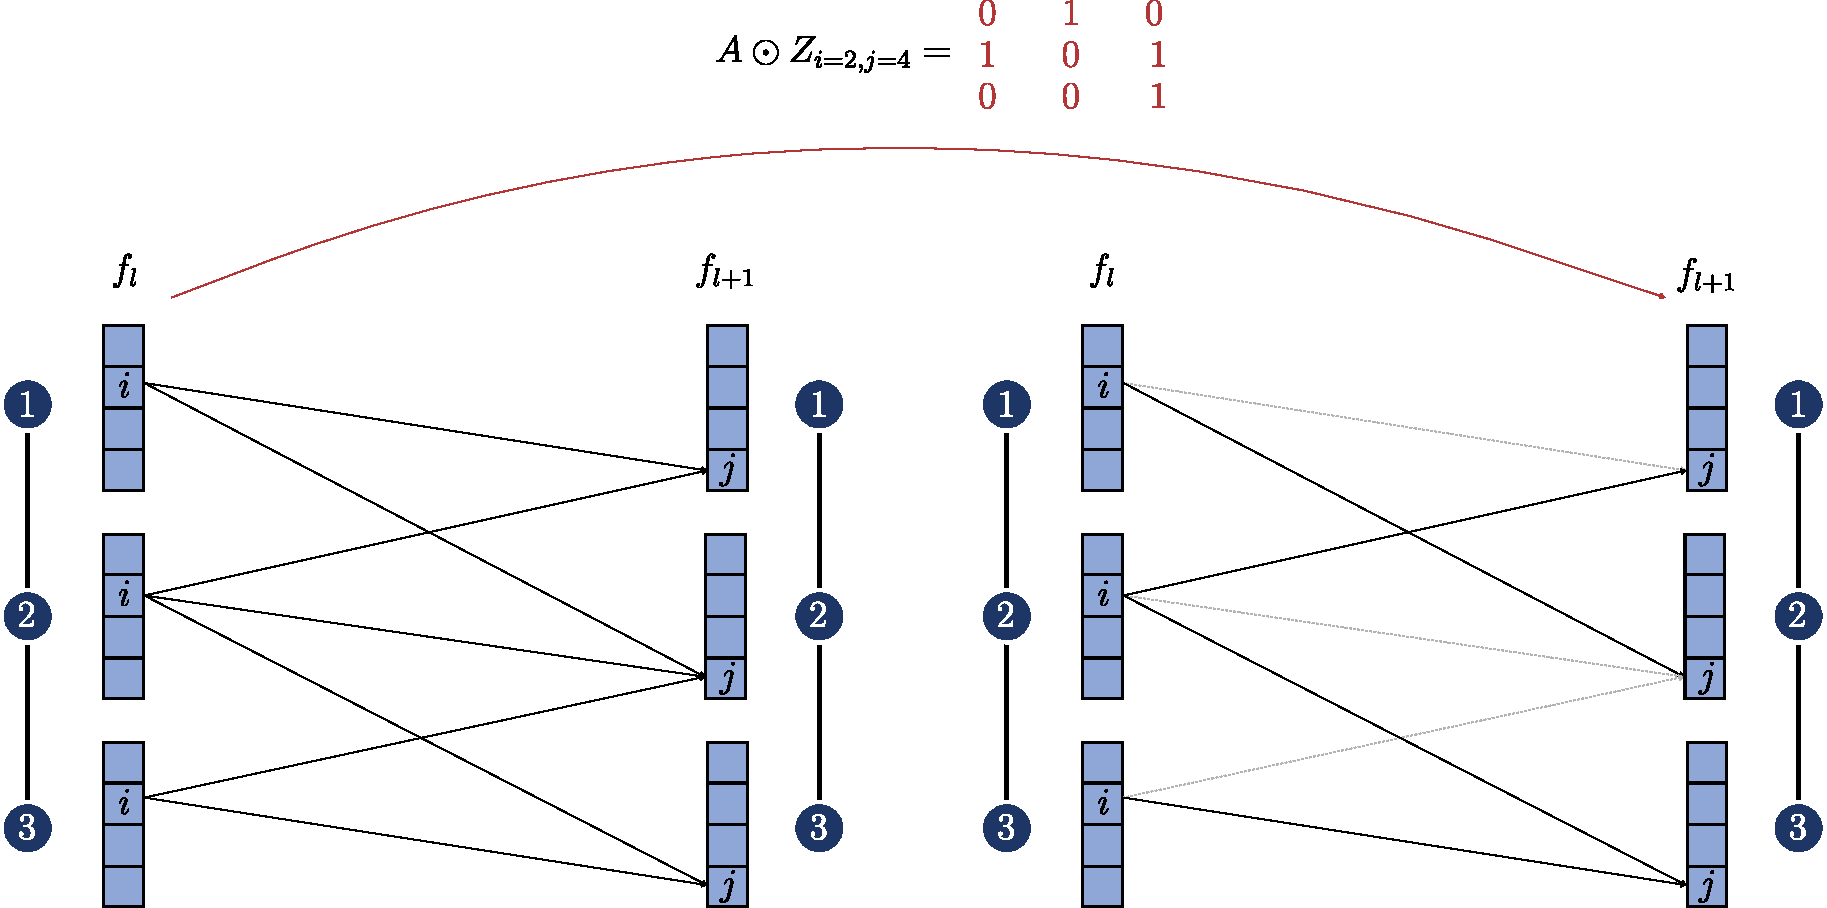
\includegraphics[width= 0.90\linewidth]{gfx/implementation/GDC-eq4.pdf}
    \caption{\Ac{gdc}Note: self connection are assumed}\label{fig:implementaion:GDC-eq4}
\end{figure}


As for the implementation of \ac{gdc}, we decided to implement the less complex version, as shown below, since this implementation reduces the runtime completely and is also the one that was originally implemented for testing the efficacy of \ac{gdc}

\begin{align}
    H^{(l+1)} = \sigma(\sum_{i= 1}^{f_{l}}\mathfrak{N}(A \odot Z_{i}^{(l)})H^{(l)}[:,i] W^{(l)}[i,:]) \label{eq:relaxed}
\end{align}



Here, we compute the new feature matrix in one go instead of doing $f_{l}$ iterations for all $f_{l}$ columns.
\begin{figure}[ht]
    \centering
    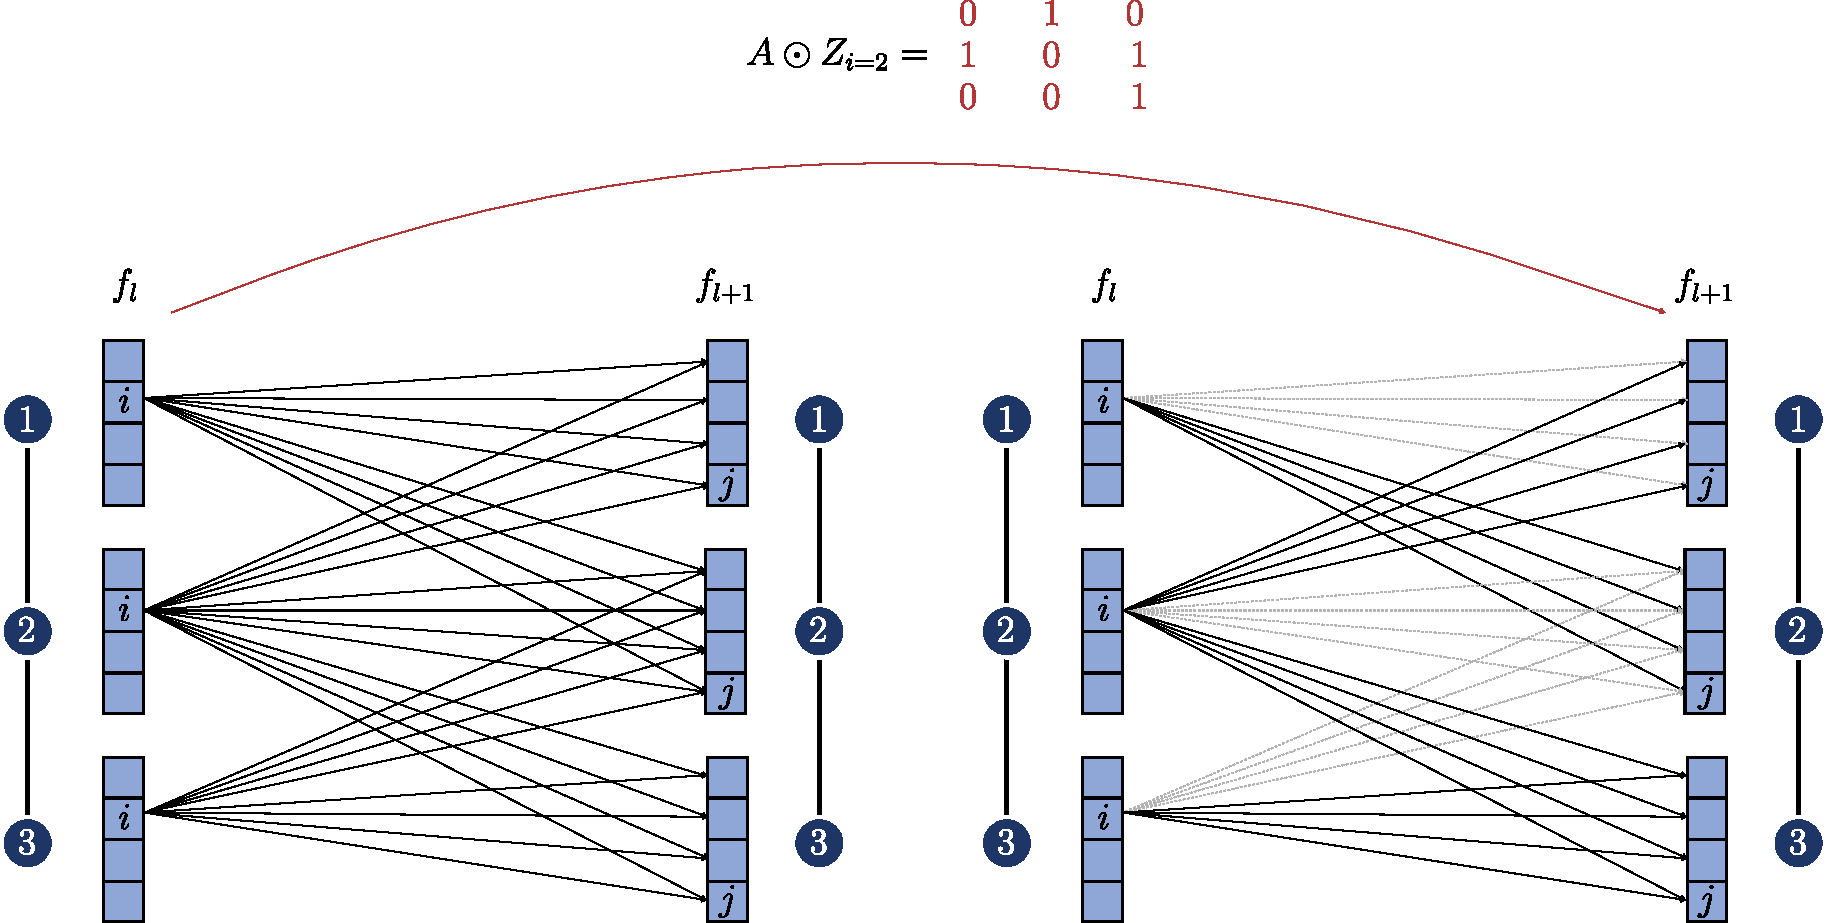
\includegraphics[width= 0.90\linewidth]{gfx/implementation/GDC-eq5.pdf}
    \caption{Originally proposed \ac{gdc}Note: self connection are assumed}\label{fig:implementaion:GDC-eq5}
\end{figure}




% Implementation of Regularization 
The four regularization techniques, as described in \ref{sec:related:pred:regularization}, can be described using two parameters illustrated in the table below: Is the regularization happening row-wise, and do we gather the values before applying the regularization?
\begin{center}
    \begin{tabular}{lll}
        \toprule
        \textbf{Regularization} & \textbf{row-wise?} & \textbf{gather first?} \\
        \midrule
        \acf{do}                & false              & false                  \\
        \acf{de}                & true               & true                   \\
        \acf{ns}                & true               & false                  \\
        \acf{gdc}               & false              & true                   \\

        \bottomrule
    \end{tabular}
\end{center}
\subsubsection{gather, scatter, sparcity}
In our implementation, we make use of TensorFlow gather and scatter operations:
The gather operation in TensorFlow extracts specific elements from a tensor along a given axis. Given an input tensor and a list of indices, the gather operation selects elements based on the provided indices from the input tensor. Given a tensor representing node features in a graph and a list of node indices, the gather operation extracts the corresponding node features. The gather operation can extract node features, adjacency information, or other relevant data based on specific graph node indices.

The scatter operation in TensorFlow is the inverse of the gather operation. It updates the elements of an existing tensor based on the provided indices. Given an input tensor, a list of indices, and a tensor containing values, the scatter operation replaces elements in the input tensor at the specified indices with the corresponding values from the values tensor.
Gather and scatter operations are crucial for tasks involving graph neural networks \acp{gnn} where information aggregation and dissemination across nodes are essential. Information from nodes or subgraphs is gathered and aggregated for graph classification tasks to represent the entire graph.\acp{gnn} can use gather operations to pool information from nodes and perform graph-level predictions.

\section{Choice of Frameworks}
\label{sec:implement:setup: frameworks}
Below, we briefly overview used datasets and frameworks and motivate the choice.
\subsubsection{Datasets}
\label{sec:implement:setup:frameworks: choice}
% Datasets - OGB 
Even though machine learning on graph-structured data is carried out in many areas and has many interesting use cases ranging from social networks to molecular graphs, manifolds, and source code~\cite{Hu2020},
there is no unified framework for working with graph-structured data. Furthermore, commonly used datasets and evaluation procedures suffer from multiple issues that negatively affect the quality of predictions and the reliability of evaluations of models.
Machine learning algorithms rely heavily on data. For a \ac{gnn} to be able to make accurate predictions, there is a need for a sufficient amount of properly prepared training data. Standardized splitting and evaluation methods are needed to compare different models against each other.

% Problems overview 
Today, most of the frequently used graph datasets are extremely small compared to graphs found in real applications. The same datasets, such as Cora, CiteSeer, and PubMed, are used repeatedly to train various models, leading to poor scalability in most cases. Small datasets also make it hard to rigorously evaluate data-hungry models, such as \acfp{gnn}. The performance of a \ac{gnn} on these datasets is often unstable and nearly statistically identical to each other, due to the small number of samples the models are trained and evaluated on~\cite{Kipf2017,Xu2019, Hu2020}.

% OGB benefits  
\textbf{\Ac{ogb}} offers a wide range of different-sized graph datasets from different domains for a variety of varying classification tasks and provides a unified pipeline for working with the datasets in \ac{ml} tasks.
The unified experimental protocol with standardized dataset splits, evaluation metrics, and cross-validation protocols makes it easy to compare performance reported across various studies~\cite{Hu2020}.

% Overview of standardized pipeline 
Working with \ac{ogb} consists of following steps:

\begin{enumerate}
    \item \Ac{ogb} provides realistic, different-scaled graph benchmark datasets that cover different prediction tasks from diverse applications.
    \item Dataset processing and splitting is fully automated. \Ac{ogb} data loaders automatically download and process graphs and further split the datasets in a standardized manner. This is compatible with multiple libraries and provides a library-agnostic option.
    \item This step includes developing an \ac{ml} model to train on the \ac{ogb} datasets.
    \item  \Ac{ogb} evaluates the model in a dataset-dependent manner and outputs the model performance appropriate for the task at hand.
    \item \Ac{ogb} provides public leaderboards to keep track of recent advances.
\end{enumerate}

\begin{figure}[H]
    \centering
    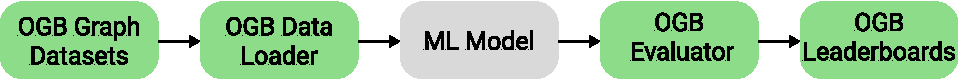
\includegraphics[width= 0.90\linewidth]{gfx/implementation/OGB_pipeline}
    \caption{\textbf{Overview of the standardized OGB pipeline} adapted from \cite{Hu2020}}\label{fig:implement:pipeline}
\end{figure}

\subsection{Finding the Best Set of Hyperparameters}
\label{sec:implement:setup: gridsearch}

For hyperparameter optimization, we use grid search \ac{gs}~\cite{Lorenzo2017,Yang2020,Zoeller2021}.\Ac{gs} is a model-free method of automated hyperparameter selection, which systematically explores the configuration space performing an exhaustive search.
\begin{enumerate}
    \item Poor scalability for large configuration spaces due to its exponential complexity in the number of hyperparameters and corresponding values. Assuming that there are k parameters, and each of them has n distinct values, its computational complexity is $O(n^{k})$
    \item Lack of consideration of the hierarchical hyperparameter structure leads to many redundant configurations.
\end{enumerate}
Despite its two major drawbacks,\ac{gs} is well-suitable for small search spaces and can easily be implemented and parallelized.